Dopo aver ripassato i numeri complessi torniamo a parlare di segnali.
\section{Terminologia}
Innanzitutto diamo prima della terminologia che ci servira' per tutta la durata del corso, in quanto valgono sia per segnali tempo-continui sia per i tempo-discreti:
\begin{itemize}
    \item SINTESI DI UN SEGNALE: composizione di segnali (solitamente) "semplici" per ottenere un segnale piu' "complesso"
    \item ANALISI DI UN SEGNALE: decomposizione di un segnale "complesso" in un insieme di segnali piu' "semplici"
\end{itemize}

Per aiutarci usiamo una formula, usando segnali a tempo continui, abbiamo un segnale tempo continuo e lo scomponiamo in composizione di somma di segnali piu' semplici ($a_k$)
\begin{equation}
    x(t) = \sum_{k = -L}^{U} a_k s(t, \xi _k)
\end{equation}

Analizzando questa espressione diciamo che il passaggio da $x(t)$ alla sommatoria e' l'operazione di analisi il cui risultato e' la combinazione lineare di $a_k, \xi_k$
Viceversa il passaggio dalla sommatoria alla funzione $x(t)$ e' l'operazione di sintesi, il cui risultato ovviamente e' $x(t)$.
La notazione $s(t, \xi_k)$ e' il segnale "semplice" o base e vediamo che non solo dipende dal tempo ma anche da un set di parametri, in questo caso chiamati $\xi_k$: $\xi_k = {f_k; \varphi_k}$, questi parametri ci permettono di comporre segnali diversi. Ad esempio il set di parametri per come abbiamo visto fino ad ora per il seno sono ampiezza, fase e frequenza.

\section{Sintesi di segnali co-sinusoidali}
Possiamo combinare linearmente segnali sinusoidali per avere segnali piu' articolati/realistici.
Vediamo un esempio:
\begin{equation}
    s(t, k) = \cos (2\pi f_k t + \varphi_k)
\end{equation}

\begin{equation}\begin{split}
    x(t) &= \frac{419}{1713} \cos (2\pi 200 t + \frac{1693}{3527} \pi) \\
    &+ \frac{629}{1069} \cos (2\pi 400 t + \frac{236}{395} \pi) \\
    &+ \frac{421}{431} \cos (2\pi 500 t - \frac{34}{917} \pi) \\
    &+ \frac{76}{279} \cos (2\pi 1600 t - \frac{232}{503} \pi) \\
    &+ \frac{89}{942} \cos (2\pi 1700 t )
\end{split}\end{equation}
Dall'esempio abbiamo tanti segnali sinusoidali che sommati danno come risultato un segnale piu'"complicato" che simula la lettere o in inglese.
Abbiamo una costante (Ampiezza) che moltiplica il coseno e dentro al coseno abbiamo una costante (frequenza) che moltiplica il tempo (t) + la fase (sempre una costante).

Quindi la sintesi ci permette di avere un segnale complicato, e sono oggettivamente simili a dei segnali reali.

Se disegniamo (tramite MatLab) il segnale risultante, otteniamo:

\begin{figure}[ht!]
    \centering
    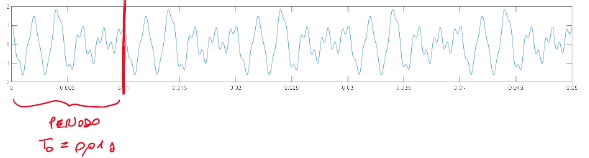
\includegraphics[scale=0.75]{immagini/lez2/esempioSintesiSegnali.jpg}
    \caption{Esempio di sintesi di segnali}
    \label{fig:esSintesiSegnali}
\end{figure}

l'unica osservazione che possiamo fare guardando il grafico e' che il periodo e' $T_0=0,01s$ ed e' quindi un segnale periodico.
Le fasi ci dicono solo come abbiamo traslato i segnali tra di loro per ottenere questa forma.

Andiamo a mettere insieme l'uso dei numeri complessi che abbiamo visto con il segnale in esempio, nonostante non ci sia nessun numero complesso c'e' il coseno e quindi possiamo usare la formula di Eulero inverso per scrivere il segnale in modo piu' compatto.
Abbiamo fatto inizialmente una sintesi:
\begin{equation}
    x(t) = \sum_{k = 1}^{5} A_k \cos (2\pi f_k t + \varphi_k)
\end{equation}

Tutti i valori con k sono dei numeri. 
Prendiamo uno degli elementi di prima, che posso scrivere con la formula di Eulero inversa del coseno.
$\theta$ e' tutto quello che c'e' nelle parentesi del coseno.

\begin{equation}
    A_k \cos (2\pi f_k t + \varphi_k) = \frac{A_k}{2} {e^{i(2\pi f_k t + \varphi_k)} + e^{-i(2\pi f_k t + \varphi_k)} }
\end{equation}

Se io adesso faccio un cambio di notazione:
\begin{equation}\begin{split}
    &\frac{A_k}{2} = a_k \\
    &f-k = -f_k
\end{split}\end{equation}

Riscriviamo quindi il nostro pezzo di segnale con la nuova notazione:
\begin{equation}
    = a_k e ^{i 2\pi f_k t} e^{i \varphi_k} + a_k e ^{-i 2\pi f_k t} e^{-i \varphi_k}
\end{equation}

Notiamo che:
\begin{equation}\begin{split}
    &a_k e^{i \varphi_k} = b_k \\
    &a_k e^{-i \varphi_k} = b_k^{\circ}
\end{split}\end{equation}

Sono uno un numero complesso e l'altro il suo coniugato, perche' il modulo ($a_k$) e' uguale per tutti e due mentre la fase cambia di segno.
Posso anche notare che c'e' un $-f_k$ che trasformo in $f-k$.
In forma compatta quindi posso dire che il segnale e':
\begin{equation}
    b_k e^{i 2\pi f_k t} + b_k^{*} e^{i 2\pi f_k t}
\end{equation}
Estendo ulteriormente la notazione e chiamo $b-k = b_k^{*}$. Tutto questo perche' voglio scrivere questo come due pezzi di un indice.

Riassumendo ho scritto:
\begin{equation}\begin{split}
    x(t) &= \sum_{k = 1}^{5} A_k \cos (2\pi f_k t + \varphi_k) \\
    &= \sum_{k = -5, k \neq 0}^{5} b_k e{i 2 \pi f_k t}
\end{split}\end{equation}

Questo passaggio lo possiamo fare se:
\begin{equation}\begin{split}
    &b-k = b_k^* \\
    &\frac{A_k}{2} e^{i \varphi_k} = b_k \\
    &-f_k = f-k
\end{split}\end{equation}

La seconda quantita' ($b_k$) e' il FASORE, ed e' solo un numero complesso in rappresentazione polare, perche' si risalta la fase.

\section{Spettro del segnale}
Lo spettro del segnale e' una rappresentazione del segnale basato sull'enumerazione di frequenza e fasore.

Vediamo come e' rappresentato un segnale:
\begin{equation}
    \{ (f_{-n}; n_{-n})(f_{-n+1}; b_{-n+1}) \mbox{...} (f_0; b_0); (f_1, b_1) \mbox{...} (f_n, b_n) \}
\end{equation}

Se usiamo la rappresentazione vista prima possiamo riscrivere la funzione come N frequenze, N fasori e tutti i coniugati complessi piu' l'elemento zero:
\begin{equation}
    \{ (-f_n; b_n^*)(-f_{n+1}; b^*_{-n+1}) \mbox{...} (0; b_0); (f_1, b_1) \mbox{...} (f_n, b_n) \}
\end{equation}

Lo spettro e' l'input che diamo per sintetizzare il segnale, e' quindi utile modificare e fare delle operazioni sullo spettro perche' modificando lo spettro viene modificato il segnale che andiamo a sintetizzare.

\subsubsection{Esempio}
Abbiamo 3 modi per rappresentare lo spettro:
\begin{itemize}
    \item Elencando i segnali che lo compongono per enumerazione
    \item Graficamente costruendo due grafici:
    \begin{itemize}
        \item Uno per il modulo 
        \item Uno per la fase
    \end{itemize}
    \item Graficamente costruendo due grafici:
    \begin{itemize}
        \item Uno per la parte reale
        \item Uno per la parte immaginaria
    \end{itemize}
\end{itemize}

Vediamo un esempio, inizialmente abbiamo un segnale rappresentato come sommatoria (un segnale sintetizzato):
\begin{equation}
    \sum_{k = -2}^{2} b_k e^{i 2 \pi f_k t}
\end{equation}

Andiamo ora ad elencare tutti i valori che $b_k$ (sono valori che ci ha dato lui), non c'e' bisogno di farlo per i negativi, perche' saranno gli opposi, o i complessi coniugati per le fasi:

\begin{equation}\begin{split}
   k=2 &\rightarrow 3 e^{i \frac{\pi}{2}} \\
   k=1 &\rightarrow \frac{1}{2} e^{-i \frac{\pi}{3}} \\
   k=0 &\rightarrow 4 \\
\end{split}\end{equation}

Ora facciamo la stessa cosa per i valori di $f_k$:

\begin{equation}\begin{split}
   k=2 &\rightarrow 250 \mbox{Hz} \\
   k=2 &\rightarrow 30 \mbox{Hz} \\
   k=2 &\rightarrow 0 \mbox{Hz} \\
\end{split}\end{equation}

Ora ricaviamo lo spettro di questo segnale scrivendolo inizialmente per enumerazione, accoppiando le frequenze ed i loro fasori, notando che dobbiamo accoppiare le frequenze negative con i fasori coniugati di quelli che abbiamo ricavato precedentemente:
\begin{equation}
    \{ (-250 \mbox{Hz}; 3e^{-i\frac{\pi}{2}}); (-30 \mbox{Hz}; \frac{1}{2}e^{i\frac{\pi}{3}}); (0 \mbox{Hz}; 4); (250 \mbox{Hz}; 3e^{i\frac{\pi}{2}}); (30 \mbox{Hz}; \frac{1}{2}e^{-i\frac{\pi}{3}}) \}
\end{equation}

Da questa rappresentazione enumerativa ricaviamo la prima rappresentazione grafica, in un grafico mettiamo tutti i moduli, mentre nel secondo grafico rappresentiamo le fasi.
Sull'asse delle x abbiamo tutte le frequenze, mentre sull'asse verticale nel caso del primo grafico rappresentiamo il numero che moltiplica il fasore (il modulo nella rappresentazione polare dei numeri complessi), mentre nel secondo grafico sull'asse delle x abbiamo sempre le frequenze, mentre sull'asse delle y abbiamo la fase (ovvero il numero che moltiplica i):

\begin{figure}[ht!]
    \centering
    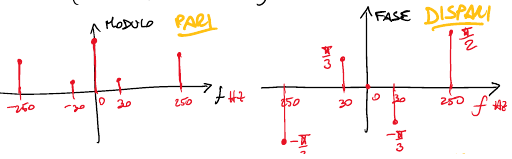
\includegraphics{immagini/lez3/moduloFase.jpg}
\end{figure}

Notiamo in questa rappresentazione che ci sono delle simmetrie:
\begin{itemize}
    \item Il modulo e' una funzione pari: ovvero che e' simmetrica rispetto all'asse y
    \item la fase e' una funzione dispari: ovvero che e' simmetrica rispetto all'origine degli assi
\end{itemize}

Esiste anche una rappresentazione in cui in un grafico rappresentiamo la parte reale mentre nell'altro la parte immaginaria. 
Come prima sull'asse x abbiamo le frequenze, mentre per mettere i punti sull'asse delle y devo prima trasformare i numeri complessi nella loro forma cartesiana, utilizzando la formula di Eulero. Ancora una volta troviamo solo i positivi e poi per i negativi semplicemente invertiamo il segno:

\begin{equation}\begin{split}
    &3e ^{i\frac{\pi}{2}} = 3(\cos \frac{\pi}{2} + i \sin \frac{\pi}{2}) = 3i \\
    &\frac{1}{2} e ^{-i\frac{\pi}{3}} = \frac{1}{2}[\cos(-\frac{\pi}{3}) + i \sin(\frac{-\pi}{3})] = \frac{1}{4} -i\frac{\sqrt{3}}{4}
\end{split}\end{equation}

\begin{figure}[ht!]
    \centering
    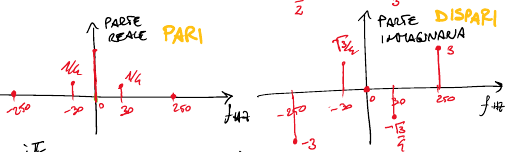
\includegraphics{immagini/lez3/realeImmaginaria.jpg}
\end{figure}

\subsection{Proprieta' dello spettro}
Vediamo come e' possibile manipolare un segnale attraverso la manipolazione dello spettro, utilizzando delle proprieta' dello spettro.

\subsubsection{Moltiplicazione per una costante}

\begin{equation}
  \textcolor{red}{C} x(t) =  \sum_{k = -n}^{n} \textcolor{red}{C}b_k e^{i 2 \pi f_k t}
\end{equation}

Quando moltiplico un segnale per una costante \textcolor{red}{C} lo spettro rimane uguale ma i fasori vengono moltiplicati per la costante stessa.

Spettro:
\begin{equation}
    \{ (-f_n; \textcolor{red}{C}b_n^*)(-f_{n+1}; \textcolor{red}{C}b^*_{-n+1}) \mbox{...} (0; \textcolor{red}{C}b_0); (f_1, \textcolor{red}{C}b_1) \mbox{...} (f_n, \textcolor{red}{C}b_n) \}
\end{equation}

\subsubsection{Somma di una costante}
QUando moltiplico un segnale per una costante \textcolor{red}{C}, lo spettro rimane uguale con l'unica differenza che il fasore dell'elemento 0 viene sommato alla costante \textcolor{red}{C}.

\begin{equation}
   x(t) + \textcolor{red}{C} =  \sum_{k = -n}^{n} b_k e^{i 2 \pi f_k t} + \textcolor{red}{C} e^{i 0}
\end{equation}

\begin{equation}
    \{ (-f_n; b_n^*)(-f_{n+1}; b^*_{-n+1}) \mbox{...} (0; b_0 + \textcolor{red}{C}); (f_1, b_1) \mbox{...} (f_n, b_n) \}
\end{equation}

\subsubsection{Somma di due segnali}
Sommare due segnali (con frequenze diverse) significa combinare i due segnali, ovvero prendere tutte le coppie (da entrambi i segnali) che hanno frequenze diverse, nel caso in cui ci sono frequenze uguali dei due segnali, si sommano i fasori di quelle frequenze.

\begin{equation}\begin{split}
    &x(t) = \{ (-f_n; b_n^*)(-f_{n+1}; b^*_{-n+1}) \mbox{...} (0; b_0); (f_1, b_1) \mbox{...} (f_n, b_n) \} \\
    &y(t) = \{ (-g_n; d_n^*)(-g_{n+1}; d^*_{-n+1}) \mbox{...} (0; d_0); (g_1, d_1) \mbox{...} (g_n, b_n) \} \\
\end{split}\end{equation}

Facciamo un esempio, consideriamo come $x(t)$ il segnale con lo spettro di prima, mentre definiamo lo spettro di $y(t)$ per enumerazione:

\begin{equation}
    \{ (-125 \mbox{Hz}; 2e^{i\frac{\pi}{2}}); (-30 \mbox{Hz}; \frac{2}{3}e^{i\frac{\pi}{4}}); (125 \mbox{Hz}; 2e^{-i\frac{\pi}{2}}); (30 \mbox{Hz}; \frac{2}{3}e^{-i\frac{\pi}{4}}) \}
\end{equation}

Applichiamo quello detto prima e facciamo la composizione dei due spettri:

\begin{equation}\begin{split}
    S_{\textcolor{red}{x + y}} =  &\{ (-250 \mbox{Hz}; 3e^{-i\frac{\pi}{2}}); (-125 \mbox{Hz}; 2e^{i\frac{\pi}{2}}); (-30 \mbox{Hz}; \frac{2}{3}e^{i\frac{\pi}{4}} + \frac{1}{2}e^{i\frac{\pi}{3}}); (0 \mbox{Hz}; 4); \\
     &(250 \mbox{Hz}; 3e^{i\frac{\pi}{2}}); (125 \mbox{Hz}; 2e^{-i\frac{\pi}{2}}); (30 \mbox{Hz}; \frac{2}{3}e^{-i\frac{\pi}{4}} + \frac{1}{2}e^{-i\frac{\pi}{3}}) \}
\end{split}\end{equation}


\subsubsection{Traslazione nel tempo}
Traslare nel tempo una funzione co-sinusoidale, come gia' abbiamo visto, significa sommare o sottrarre l'argomento della funzione per una costante $\tau$. 
Quello che succede e' che lo spettro rimane uguale, ma i fasori vengono moltiplicati, per un cosiddetto "termine di fase" che dipende dalla frequenze e non dal tempo.  Quindi cambia la fase del numero complesso ma non cambia il modulo.

Quello che ci stiamo chiedendo e' cosa succede in questo caso:
\begin{equation}\begin{split}
    &x(t) \leftrightarrow S_x \\
    &y(t) = x(t - \textcolor{red}{\tau}) \leftrightarrow S_y \mbox{?}
\end{split}\end{equation}

Cominciamo calcolando $y(t)$ esplicitamente:
\begin{equation}\begin{split}
     y(t) &=  \sum_{k = -n}^{n} b_k e^{i 2 \pi f_k (t - \textcolor{red}{\tau})} \\
\end{split}\end{equation}

Da cui otteniamo lo spettro:

\begin{equation}
    \{ (-f_n; b_n^* e^{i 2 \pi f_k  \textcolor{red}{\tau}}) \mbox{...} (0; b_0 \cdot 1); \mbox{...} (f_n, b_n e^{i 2 \pi f_k \textcolor{red}{\tau}}) \}
\end{equation}

\subsubsection{Moltiplicazione per un esponenziale complesso}
Moltiplicare un segnale per un esponenziale complesso significa trasformare il segnale in un numero costante che dipende dal tempo ma non e' un segnale reale. Quello che succede e' che le frequenze vengono spostate (sommate o sottratte) del numero. 
Notiamo che e' l'unica proprieta' che modifica le frequenze.

Ricordiamo che:
\begin{itemize}
    \item Se moltiplichiamo per un numero negativo il segnale verra' spostato verso destra
    \item Se moltiplichiamo per un numero positivo il segnale verra' spostato verso sinistra
\end{itemize}

\begin{equation}\begin{split}
     y(t) &=  \sum_{k = -n}^{n} b_k e^{i 2 \pi f_k t} e^{i 2 \pi \Tilde{f} t}\\
     &= \sum_{k = -n}^{n} b_k e^{i 2 \pi (f_k = \Tilde{f}) t}
\end{split}\end{equation}

Da cui otteniamo lo spettro per enumerazione:
\begin{equation}
    \{ (-f_n \textcolor{red}{+ \Tilde{f}}; b_n^*)(-f_{n+1} \textcolor{red}{+ \Tilde{f}}; b^*_{-n+1}) \mbox{...} (0 \textcolor{red}{+ \Tilde{f}}; b_0); (f_1 \textcolor{red}{+ \Tilde{f}}, b_1) \mbox{...} (f_n \textcolor{red}{+ \Tilde{f}}, b_n) \}
\end{equation}

Vediamo come ulteriore prova del fatto che moltiplicando per un esponenziale complesso si ottiene un segnale non reale il fatto che se tracciamo i garfici di modulo e frequenza questi non sono piu' simmetrici:

\begin{figure}
    \centering
    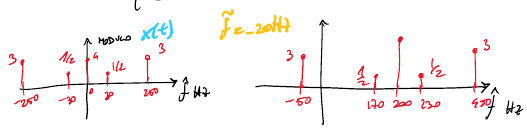
\includegraphics{immagini/lez3/molitplicazioneEsponenzialeComplesso.jpg}
\end{figure}

\section{Modulazione di ampiezza}
La modalita' di trasmissione di un segnale in modulazione d'ampiezza e' quella utilizzata dalle radio AM, che trasmettono in modulazione di ampiezza per poter aumentare di molto le frequenze di trasmissione, cosi' facendo i segnali evitano disturbi di frequenze.

Vediamo come "modulare" un segnale, immaginiamo che il segnale che vogliamo trasmettere sia x(t) e questo che viene trasmesso e' x(t) che e' l'AMPIEZZA, mentre il coseno e' la portante e $\Tilde{f}$ e' la frequenza a cui dobbiamo sintonizzarci per ascoltare i segnale:

\begin{equation}
    y(t) = x(t) \cos (2\pi \Tilde{f} t)
\end{equation}

Che spettro avra' il segnale trasmesso? per farlo utilizziamo le proprieta' che abbiamo appena visto, otteniamo questa cosa applicando il teorema di Eulero inverso del coseno:

\begin{equation}
    y(t) = x(t) \{ \frac{e}{2}^{i 2 \pi \Tilde{f} t} + \frac{e}{2}^{-i 2 \pi \Tilde{f} t}  \}
\end{equation}

Vediamo che in questa equazione abbiamo delle proprieta' che abbiamo appena visto:
\begin{itemize}
    \item La proprieta' di somma di una costante C, in questo caso $C = \frac{1}{2}$
    \item La proprieta' di somma di due segnali, perche' appunto i due esponenziali si sommano
    \item La proprieta' di moltiplicazione per un esponenziale complesso, che e' $\Tilde{f}$ 
\end{itemize}

Lo spettro finale sara' quindi dato dall'unione di tutti i segnali dei due insiemi spostato di $\Tilde{f}$ e moltiplicato per $\frac{1}{2}$ (ovvero tutti i fasori saranno moltiplicati per $\frac{1}{2}$).

E se tracciamo i grafici di modulo e frequenza vediamo che viene modificata la frequenza e quindi l'ampiezza del segnale.
Nel nostro caso consideriamo $\Tilde{f} = 1000 \mbox{Hz}$ e notiamo che il tutti i punti del grafico vengono traslati di 1000 posizioni.

\begin{figure}[ht!]
    \centering
    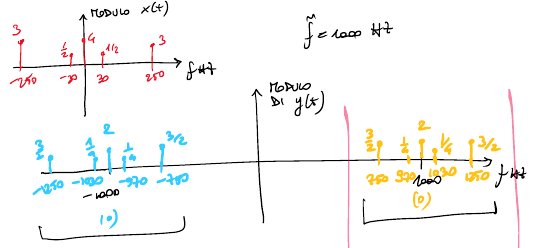
\includegraphics{immagini/lez3/modulazioneAmpiezza.jpg}
\end{figure}

\section{Esercizio di sintesi}
Dato il seguente spettro:

\begin{equation}
    \{ (-3 \mbox{Hz}; 1 + i\sqrt{3}),(-2 \mbox{Hz}; \frac{\sqrt{3}}{2} - i \frac{1}{2}),(0 \mbox{Hz}; 3),(2 \mbox{Hz}; \frac{\sqrt{3}}{2}  i \frac{1}{2}),(3 \mbox{Hz}; 1 + i\sqrt{3}) \}
\end{equation}

Calcoliamo qual'e' il segnale $x(t)$ a cui appartiene.
Innanzitutto notiamo che il segnale e' un segnale reale, in quanto tutti i segnali che lo compongono sono a coppie ed i fasori sono complessi coniugati tra di loro, ed inoltre sono in forma cartesiana, quindi li trasformiamo in forma polare:

\begin{equation}\begin{split}
    &z = 1 \pm i \sqrt{3}: \\
    &\rho = \sqrt{i^2 + \sqrt{3}^2} = 2 \\
    &\theta = arctan \frac{\pm \sqrt{3}}{1} = \pm \frac{\pi}{3}\\
    &z = 2 e^{\pm i \frac{\pi}{3}}
\end{split}\end{equation}

\begin{equation}\begin{split}
    &z = : \frac{\sqrt{3}}{2} \pm i \frac{1}{2}\\
    &\rho = \sqrt{(\frac{\sqrt{3}}{2})^2 + (\pm i \frac{1}{2})^2} = 1 \\
    &\theta = arctan \frac{\pm \frac{1}{2}}{\frac{\sqrt{3}}{2}} = arctan \frac{1}{\sqrt{3}} = \pm \frac{\pi}{6} \\
    &z = 1 e^{\pm i \frac{\pi}{6}}
\end{split}\end{equation}

Ora semplicemente copiamo ed incolliamo le frequenze ed i fasori, secondo la formula che abbiamo visto prima:

\[\begin{split}
    x(t) &=\{ (-3 \mbox{Hz}; 2e^{i \frac{\pi}{3}} \cdot e^{-i2 \pi 3 t}) + (-2 \mbox{Hz}; e^{-i \frac{\pi}{6}} \cdot e^{-i2 \pi 2 t}) + (0 \mbox{Hz}; 3e^{i 0} \cdot e^{-i2 \pi 0 t}) \\
    &+ (2 \mbox{Hz}; e^{i \frac{\pi}{6}} \cdot e^{-i2 \pi 2 t}) + (3 \mbox{Hz}; 2e^{-i \frac{\pi}{3}} \cdot e^{-i2 \pi 3 t}) \}
\end{split}\]

A questo punto mettiamo insieme gli esponenti degli esponenziali moltiplicati tra di loro, inoltre raccogliamo la i e portiamo fuori i meno in modo tale che gli esponenziali con la stessa base siano complessi coniugati per poter applicare la formula di Eulero:

\[\begin{split}
    2e^{-i(2\pi 3t - \frac{\pi}{3}} + e^{-i(2\pi 2t + \frac{\pi}{3}} + 3 + e^{i(2\pi 2t + \frac{\pi}{6}} + 2e^{i(2\pi 3t - \frac{\pi}{3}}
\end{split}\]

Applichiamo la formula di Eulero tra i coniugati ed ottieniamo:

\[
    4 \cos{(2\pi 3t - \frac{\pi}{3})} + 2 \cos{(2\pi 2t +\frac{\pi}{6})} + 3
\]

Ora dobbiamo trovare qual'e' lo spettro del segnale $y(t) = x(t - 10)$ e va derivato dallo spettro di $x(t)$. Sappiamo che si tratta di una traslazione nel tempo, quindi semplicemente applichiamo la regola vista in precedenza della traslazione nel tempo. Ricordando che vanno moltiplicati i fasori per la costante.
Quello che facciamo e' prendere lo spettro che precedentementa avevamo modificato portando le fasi in rappresentazione polare e moltiplichiamo la costante ai fasori:

\[\begin{split}
    x(t) &=\{ (-3 \mbox{Hz}; 2e^{i \frac{\pi}{3}} \cdot e^{-i2 \pi 3 \textcolor{red}{10}}) + (-2 \mbox{Hz}; e^{-i \frac{\pi}{6}} \cdot e^{-i2 \pi 2 \textcolor{red}{10}}) + (0 \mbox{Hz}; 3e^{i 0} \cdot e^{-i2 \pi 0 \textcolor{red}{10}}) \\
    &+ (2 \mbox{Hz}; e^{i \frac{\pi}{6}} \cdot e^{-i2 \pi 2 \textcolor{red}{10}}) + (3 \mbox{Hz}; 2e^{-i \frac{\pi}{3}} \cdot e^{-i2 \pi 3 \textcolor{red}{10}}) \}
\end{split}\]
%non l'ho finito perche' non mi sembra sensato copiare gli esercizi, li terro' sul quaderno

\section{Terminologia}
Diamo delle definizioni in modo da avere un base terminologica:
\begin{itemize}
    \item Frequenze armoniche: sono tutti i multipli interi di una frequenza detta frequenza fondamentale $F_0$.
\end{itemize}

Se ad esempio la frequenza base $F_0 = 10$ Hz, la $3^a$ armonica sarebbe 30 Hz e cosi' via.

\section{Teorema della serie di Fourier}
Cominciamo notando che partendo da una frequenza $F_0$ nota, moltiplicandola per una costante $k \in \mathbf{R}$ crescente, il periodo $T_0$ del segnale diminuisce, in particolare $\cos{(s\pi k F_0 t)}$ avra' periodo $T= \frac{1}{k \cdot T_0} = \frac{1}{k} T_0$.
Questa cosa ci fa capire che se uso frequenze armoniche di $F_0$ sicuramente sono periodiche anche per il periodo base $T_0$. Di conseguenza se faccio la sintesi tra frequenze armoniche sicuramente so che il segnale risultante sia periodico:
\begin{equation}
    \mbox{Se } f_k = k F_0 \Leftrightarrow x(t) = \sum_{k} b_k e^{i 2 \pi f_k t} \mbox{PERIODICO}
\end{equation}

Il viceversa, ovvero che se scindo un segnale periodico posso scriverlo come combinazione di infinite frequenze armoniche si chiama teorema sulle serie di Fourier:
$x(t)$ e' un segnale (TEMPO CONTINUO) periodico di periodo $T_0$ puo' essere sintetizzato come:
\begin{equation}
    \mbox{SINTESI: }x(t) = \sum_{k = - \infty}^{+ \infty} a_k e^{\textcolor{red}{+} j 2\pi F_0 k t} \rightarrow F_0 = \frac{1}{T_0}
\end{equation}

dove

\begin{equation}
    \mbox{ANALISI: } a_k = \frac{1}{T_0} \int_0^{T_0} x(t) e^{\textcolor{red}{-} j 2\pi F_0 k t} dt
\end{equation}

Ricordiamoci che se la sintesi deve dare un segnale reale ogni $a_k$ deve avere un suo complesso coniugato ed in particolare $a_k^* = a-k$.

Inoltre che il segnale $a_0$ sara' dato da $\frac{1}{T_0} \int_0^{T_0} x(t) \cdot 1 dt$, ovvero l'integrale del segnale nel periodo.

\subsection{Spettro di un segnale periodico}
Come ci aspettiamo lo spettro di un segnale periodico avra' infinite componenti.

\subsection{Esempio}
Facciamo l'analisi di un segnale periodico $x(t) = |\sin{\frac{2\pi t}{T_s}}|$.
Quello che faremo nella pratica e' rettificare un segnale sinusoidale.

Iniziamo disegnando il grafico, notiamo subito che essendo il modulo di un seno, sara' il grafico del seno con le parti negative ribaltate rispetto all'asse x.

Il seno sara' uguale a 0 quando $\frac{2\pi t}{T_s} = k\pi$ (ovvero quando l'argomento del seno e' $k \pi$), cancellando il $\pi$ ottengo che in tutti i punti $t = \frac{k T_s}{2}$, sono tutti i punti in cui il seno inteseca l'asse orizzontale.

\begin{figure}[ht!]
    \centering
    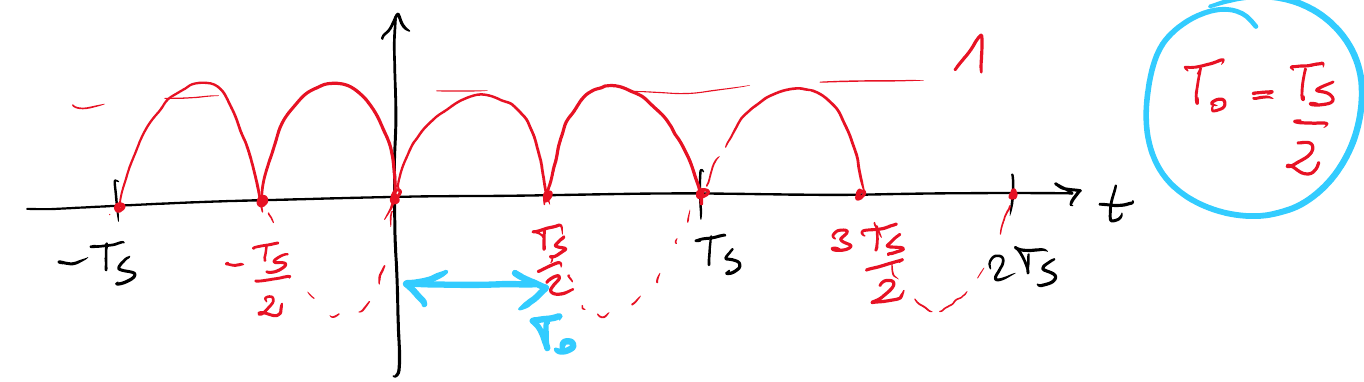
\includegraphics[scale=0.35]{immagini/lez4/grafico.jpg}
\end{figure}

Dato che e' un segnale continuo e periodico posso applicare il teorema di Fourier, ricordando prima l'unico integrale che dobbiamo ricordarci:

\begin{equation}
    \int e^{\alpha t \, dt} = \frac{1}{\alpha} e^{\alpha t}
\end{equation}

applicando il teorema di Fourier per l'analisi:

\[\begin{split}
    a_k &= \frac{1}{T_0} \int_0^{T_0} \sin{\frac{2\pi t}{T_s}} e^{-i 2\pi F_0 k t} dt \\
    &\mbox{Formula di Eulero inversa per il seno} \\
    &= \frac{1}{T_0} \int_0^{T_0} \{ \frac{e^{\frac{i 2 \pi t}{T_s}} - e^{\frac{-i 2 \pi t}{T_s}}}{2i} \} e^{-i 2\pi F_0 k t} dt \\
    &\mbox{Spezzo l'integrale} \\
    &= \frac{1}{T_0} \int_0^{T_0} \frac{e}{2i}^{\frac{i 2 \pi t}{T_s}} e^{-i 2\pi F_0 k t} dt - \frac{1}{T_0} \int_0^{T_0} \frac{e}{2i}^{\frac{-i 2 \pi t}{T_s}} e^{-i 2\pi F_0 k t} dt \\
    &\mbox{Porto fuori il denominatore, ed unisco gli esponenti con la stessa base raccogliendo la i} \\
    &= \frac{1}{2i T_0} \int_0^{T_0} e^{i (\frac{2\pi}{T_s} - 2\pi k F_0) t}dt - \frac{1}{2i T_0} \int_0^{T_0} e^{-i (\frac{2\pi}{T_s} - 2\pi k F_0) t} dt \\
    &\mbox{Applico la formula di risoluzione del logaritmo vista prima} \\
    &= \frac{1}{2i F_0} [ \frac{e^{i 2\pi (\frac{1}{T_s}- k F_0) t}}{i 2\pi (\frac{1}{T_s} - k F_0)}] - \frac{1}{2i F_0} [ \frac{e^{-i 2\pi (\frac{1}{T_s}- k F_0) t}}{-i 2\pi (\frac{1}{T_s} - k F_0)}] \\
    &\mbox{Dopo una serie di semplificazioni} \\
    &= - \frac{1}{2 \pi (1 - 2 K)} - [e^{i 2 \pi (\frac{1 - 2k}{2}) - 1}] - \frac{1}{2 \pi (1 - 2 K)} - [e^{-i 2 \pi (\frac{1 - 2k}{2}) - 1}] \\
    -1 &= e^{i \pi (1 - 2k)} \mbox{ed } e^{-i \pi (1 + 2k)} = -1 \rightarrow \forall k \in \mathbf{N} \\
    &\mbox{possiamo quindi riscrivere il segnale}\\
    a_k &= \frac{2}{2 \pi (1 - 2k)} + \frac{2}{2 \pi (1+2k)} \\
    &= \frac{2}{\pi (1 - 4 k^2)} 
\end{split}\]

Ma dato che sappiamo un segnale periodico avere infinite componenti lo scriviamo come sommatoria:

\[
    x(t) = \sum_{k = - \infty}^{+\infty} \frac{2}{\pi (1 - 4 k^2)} e^{-i 2\pi F_0 k t}
\]

\section{Condizioni sufficienti di esistenza della serie di Fourier}

Dirichlet si e' inventato delle condizioni di esistenza della serie di Fourier. Noi diremo piu' semplicemente che la serie esiste sempre, in quanto vedremo che le condizioni poste sono sufficientemente ampie, di conseguenza, dato che trattiamo segnali reali, ogni segnale che vedremo le rispettera'.

\subsection{$x(t)$ assolutamente sommabile}
Significa che e' possibile calcolare l'integrale sul periodo del segnale, il risultato dell'integrale dev'essere un numero C minore di infinito. 
E' una cosa che con i segnali reali succede sempre, non esiste un segnale che converge a piu' infinito.

\begin{equation}
    \int_0^{T_0} |x(t)| d t = C < + \infty
\end{equation}

\begin{figure}[ht!]
    \centering
    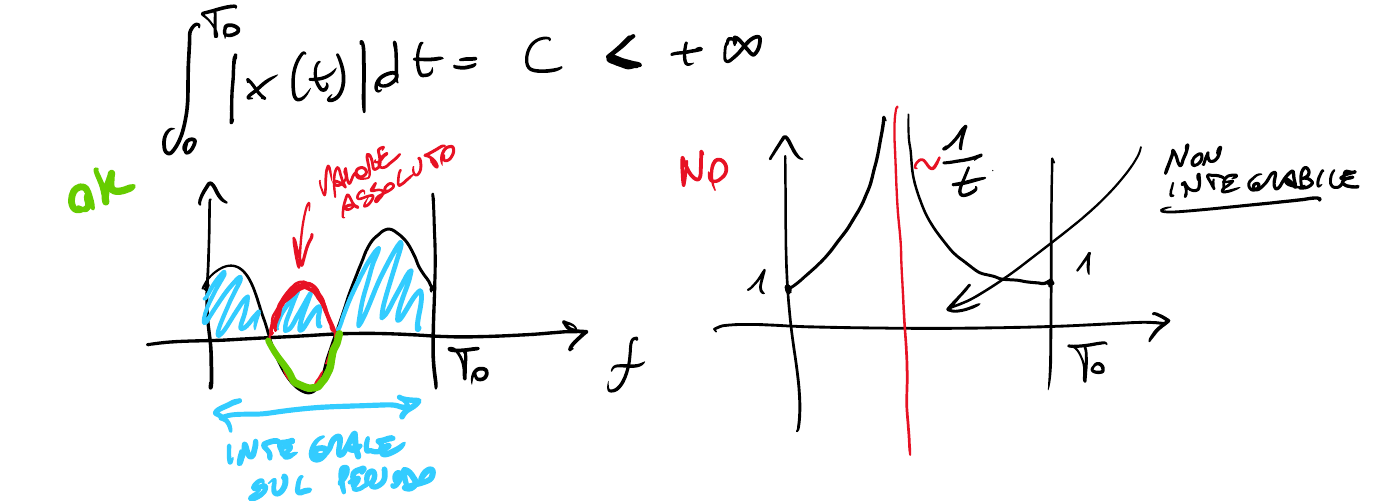
\includegraphics[scale=0.35]{immagini/lez5/assolutamenteSommabile.jpg}
\end{figure}

\subsection{$x(t)$ ha un numero finito di estremi (massimi e minimi, nel periodo)}

\begin{figure}[ht!]
    \centering
    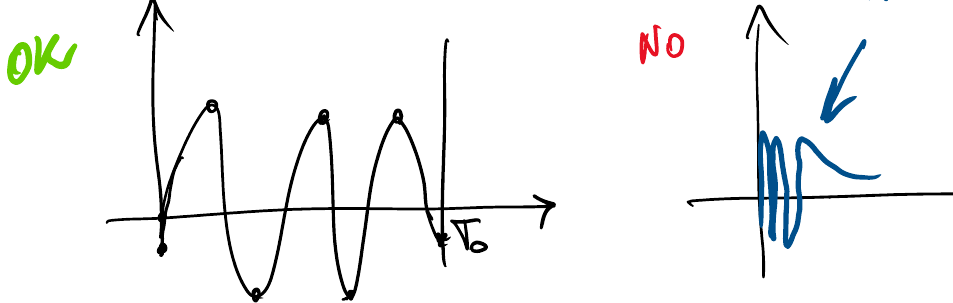
\includegraphics[scale=0.35]{immagini/lez5/finitoMassimi.jpg}
\end{figure}

I segnali che non rispettano questa proprieta' hanno un andamento del tipo $\sin{\frac{1}{x}}$ in quando oscillano infinito volte avvicinandosi ad un punto.

\subsection{$x(t)$ ha un numero di discontinuita' finite e dev'essere finito (nel periodo)}
Con discontinuita' intendiamo salti e semplicemente significa che la funzione deve avere un numero finito di salti ed ogni salto dev'essere finito.
Anche in questo caso ogni segnale reale rispetta questa proprieta'.

\begin{figure}[ht!]
    \centering
    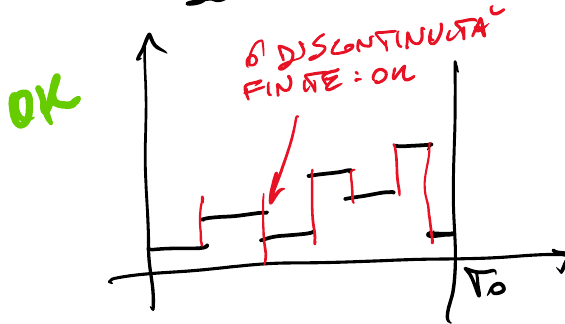
\includegraphics[scale=0.35]{immagini/lez5/discontinuitaFinite.jpg}
\end{figure}

Trovare un segnale che non rispetta questa proprieta' e' difficile, esiste pero' il segnale di cantor, che e' un segnale costruito dal seguente algoritmo:
\begin{enumerate}
    \item $T_0 = 1$ e $X_0(t) = 1$
    \item Dividi $X_i (t)$ in tre parti dove vale 1
    \item Aggiungi a quella centrale -1 per ottenere $X_i+1 (t)$
\end{enumerate}

e si ottiene questo segnale

\begin{figure}[ht!]
    \centering
    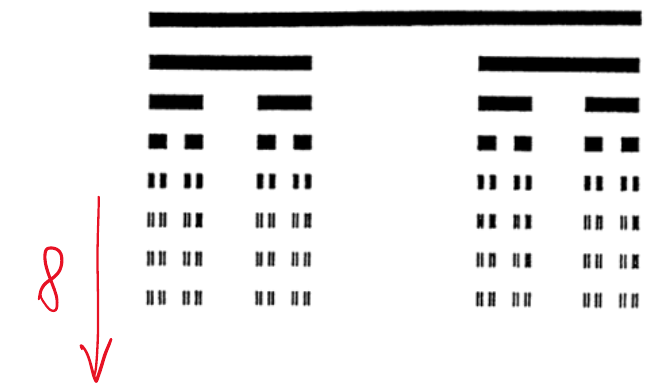
\includegraphics[scale=0.35]{immagini/lez5/cantorSet.jpg}
\end{figure}


\section{Figura di riassunto}

\begin{figure}[ht!]
    \centering
    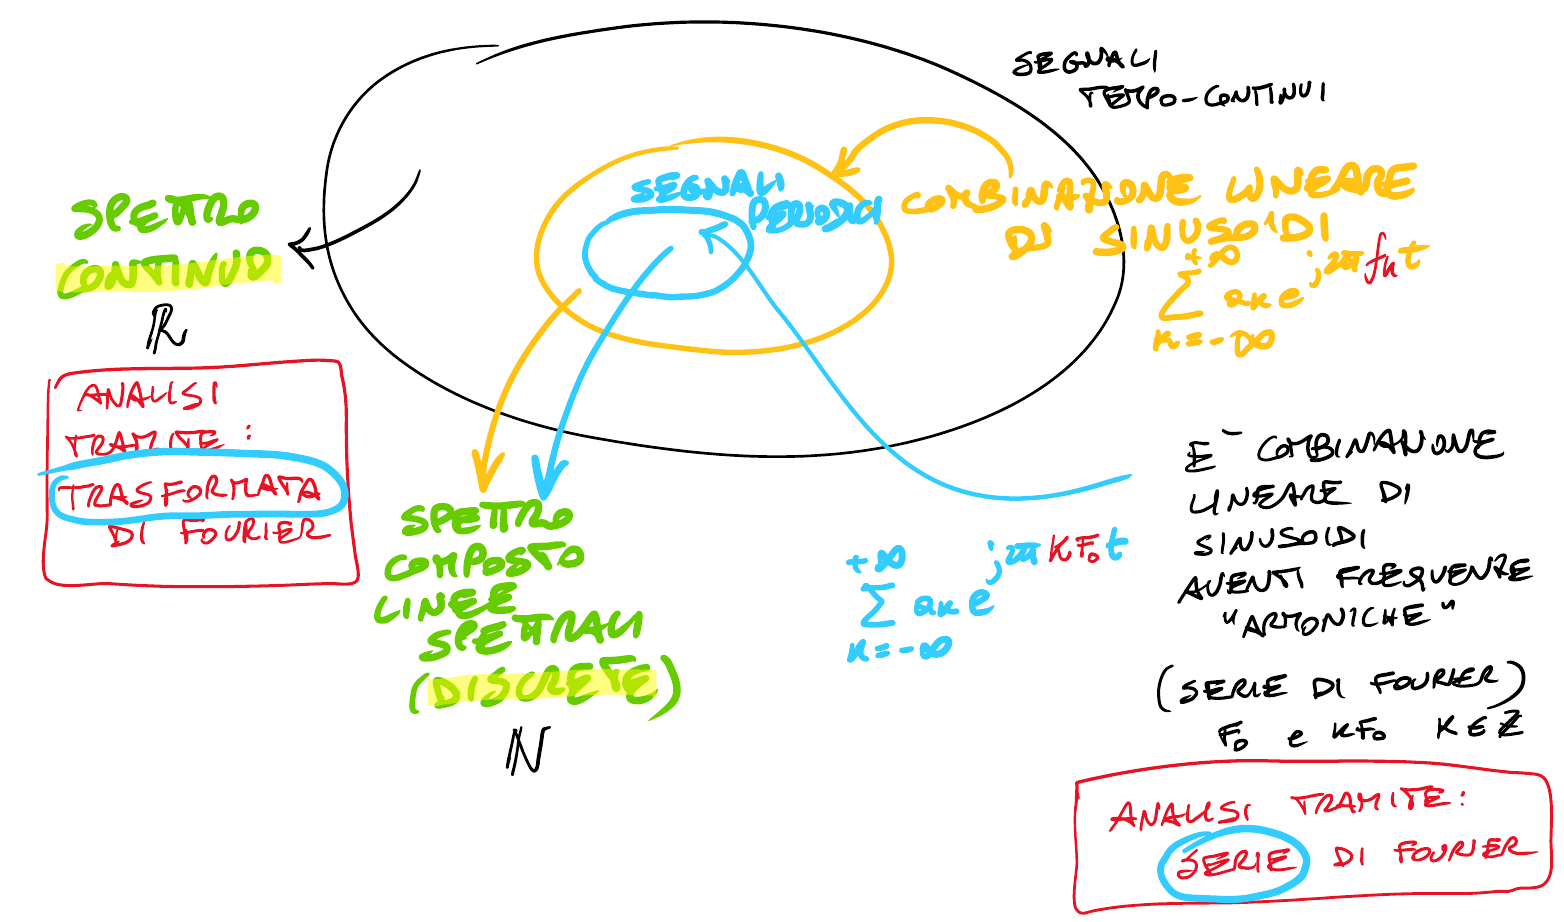
\includegraphics[scale=0.35]{immagini/lez5/schemaRiassuntivo.jpg}
\end{figure}

Si dice che i segnali appartenenti all'insieme R hanno lo spettro con la stessa potenza dei reali, allo stesso modo i segnali appartenenti all'insieme N hanno lo spettro con la stessa potenza dei numeri naturali.

\section{Trovare frequenza fondamentale date delle armoniche}
Capiamo ora quando ci viene dato un segnale composto da piu' frequenze a capire se le frequenze da cui e' composto sono armoniche.
Semplicemente date delle frequenze prendiamo il Minimo Comune Denominatore, il quale oltre a dimostrare il fatto che le frequenze sono arminche tra di loro e' anche la frequenza fondamentale $F_0$.

\subsection{Esempio 1}
Date le seguenti frequenze:
\begin{itemize}
    \item $f_1 = 16$ Hz
    \item $f_2 = 24$ Hz
    \item $f_3 = 40$ Hz
\end{itemize}

Cerchiamo di capire se sono frequenza armoniche.
Inizialmente le scomponiamo in fattori primi:
\begin{itemize}
    \item $f_1 = 2^4$
    \item $f_2 = 2^3 \cdot 3$
    \item $f_3 = 2^3 \cdot 5$
\end{itemize}

Da questa scomposizione prendiamo il MCD $2^3$ che sara' quindi la frequenza fondamente $F_0 = 2^3 \mbox{Hz}$ che ci dimostra il fatto che le frequenze sono armoniche.
Dalla frequenza fondamentale possiamo che ricavare il periodo base $T_0 = \frac{1}{8} 5$.
A questo punto possiamo esprimere le frequenze in funzione della frequenza fondamentale, dividendo la frequenza per la frequenza principale, capendo quindi di quale armonica si tratta:

\begin{itemize}
    \item $f_1 = 2 \cdot F_0 \rightarrow \, 2^a\mbox{ armonica}$
    \item $f_2 = 3 \cdot F_0 \rightarrow \, 3^a\mbox{ armonica}$
    \item $f_3 = 5 \cdot F_0 \rightarrow \, 5^a\mbox{ armonica}$
\end{itemize}

\subsection{Esempio 2}
Date le frequenze:
\begin{itemize}
    \item $f_1 = 31$ Hz
    \item $f_2 = e^1$ Hz
    \item $f_3 = \pi$ Hz
\end{itemize}

possiamo subito dire, dato che alcune frequenze sono numeri irrazionali non e' possibile che siano multipli di un numero comune, di conseguenza il segnale composto da queste frequenze non e' periodico.

\subsection{Esempio 3}
Date le frequenze:
\begin{itemize}
    \item $f_1 = \cos{(4 \pi t)}$ Hz
    \item $f_2 = \cos{(\frac{8}{5} \pi t)}$ Hz
    \item $f_3 = \cos{(\frac{16}{5} \pi t)}$ Hz
\end{itemize}

%da finire ma perche' non l'ho capito, come passa alle frazioni

\section{Esempio condizioni Fourier}

Abbiamo precedentemente trovato la serie di Fourier per il seno rettificato:

\[\begin{split}
    &x(t) = |\sin{\frac{2 \pi t}{T_s}}| \\
    &\mbox{Serie di Fourier:} \\
    &x(t) = \sum_{k = - \infty}^{+ \infty} \frac{2}{\pi (1 - 4 k^2)} e^{-j 2\pi t k \frac{2}{T_s}} \\
    &T_0 = \frac{T_s}{2}\\
    &F_0 = \frac{2}{T_s}
\end{split}\]

Tracciandone il grafico:

\begin{figure}[ht!]
    \centering
    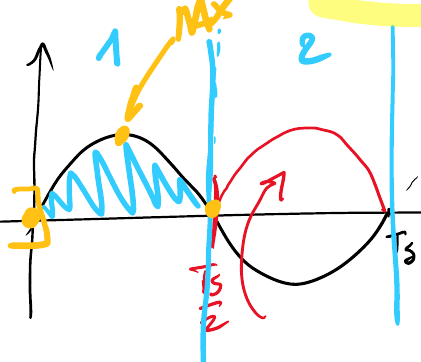
\includegraphics[scale=0.5]{immagini/lez6/sinRettificato.jpg}
\end{figure}

Ma rispetta le condizioni di esistenza?
\begin{enumerate}
    \item L'integrale nel periodo e' un numero in quanto la funzione e' finita
    \item Ho un numero finito di estremi, nel nostro caso 1 massimo ed 1 minimo
    \item Ho un numero finito di dinscontinuita', non ne ho
\end{enumerate}

Disegniamo adesso data la serie di Fouerier i grafici del segnale, del modulo e della fase.
Per farlo diamo semplicemente dei valori a k e vediamo cosa succede a $a_k$ ed a $f_k$, ricordandoci che $a_k = \frac{2}{\pi (1-4 k^2)}$ e $f_k = k F_0$.

\begin{figure}[ht!]
    \centering
    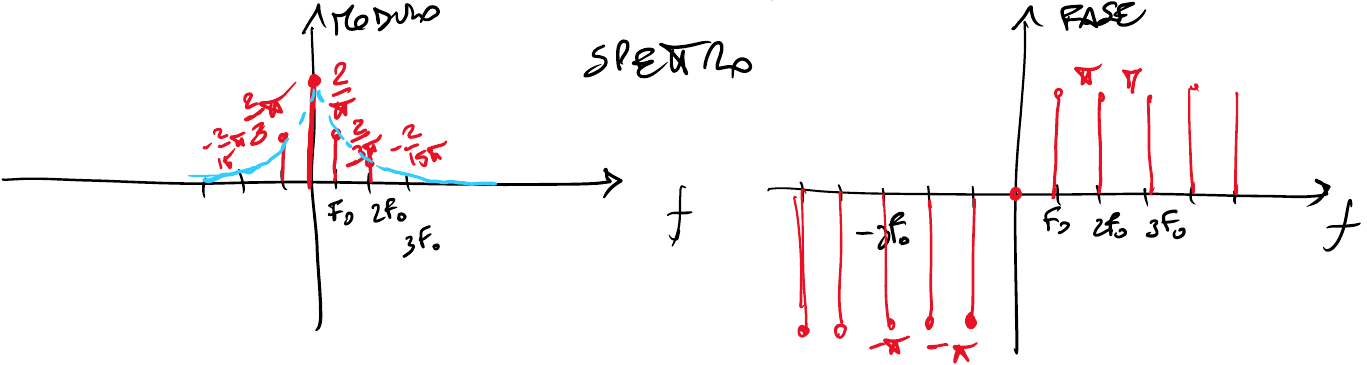
\includegraphics[scale=0.35]{immagini/lez6/moduloFaseSinRettificato.jpg}
\end{figure}

L'intuizione che abbiamo e' che dobbiamo per forza troncare la sommatoria ad un certo punto, in quanto non possiamo nella realta' continuare a sommare a $+ \infty$.

\section{Esempio Pulse Wave}

Consideriamo adesso questo segnale, chiamato Pulse Wave (o ad impulsi).
Che ha periodo $1 \rightarrow T_0$, ha la caratteristica di valere 1 per un tempo $\tau <T_0$ e 0 il resto del tempo. Inoltre un'altra caratteristica e' il duty cicle, ovvero quanto tempo e' acceso e spento (vale o 1 o 0), che e' dato da $\frac{\tau}{T_0}$.

\begin{figure}[ht!]
    \centering
    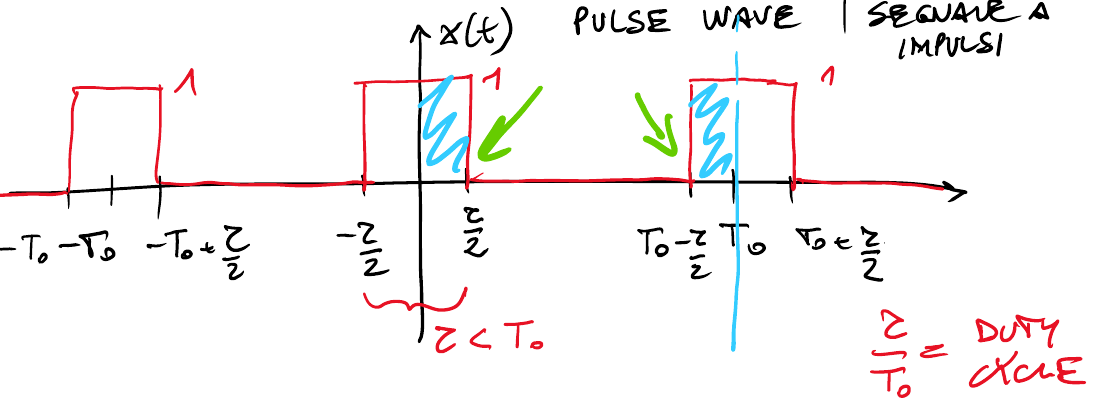
\includegraphics[scale=0.35]{immagini/lez6/pulseWave.jpg}
\end{figure}

Rispetta le condizioni di Dirichlet?
\begin{itemize}
    \item $\int_0^{T_0} |x(t)| dt = \tau < + \infty$. L'integrale nel periodo e' un numero finito
    \item Ho un numero finito di massimi e minimi, la funzione vale o 1 o 0
    \item Ho un numero finito di discontinuita', 2.
\end{itemize}

Allora se rispetta tutte le condizioni deve esistere una serie di Fourier, di cui :
\[\begin{split}
    a_k =
  \begin{cases}
    \frac{\tau}{T_0} & \text{se } k = 0 \\
    \frac{\sin{(\pi F_0 k \tau)}}{\pi k}    & \text{se } k \neq 0\\
  \end{cases}
  \, \mbox{ ed  }F_0 = \frac{1}{T_0}
\end{split}\]

Notiamo disegnando il grafico del modulo che il segnale converge a 0 piu' e' grosso il duty cicle.

\begin{figure}[ht!]
    \centering
    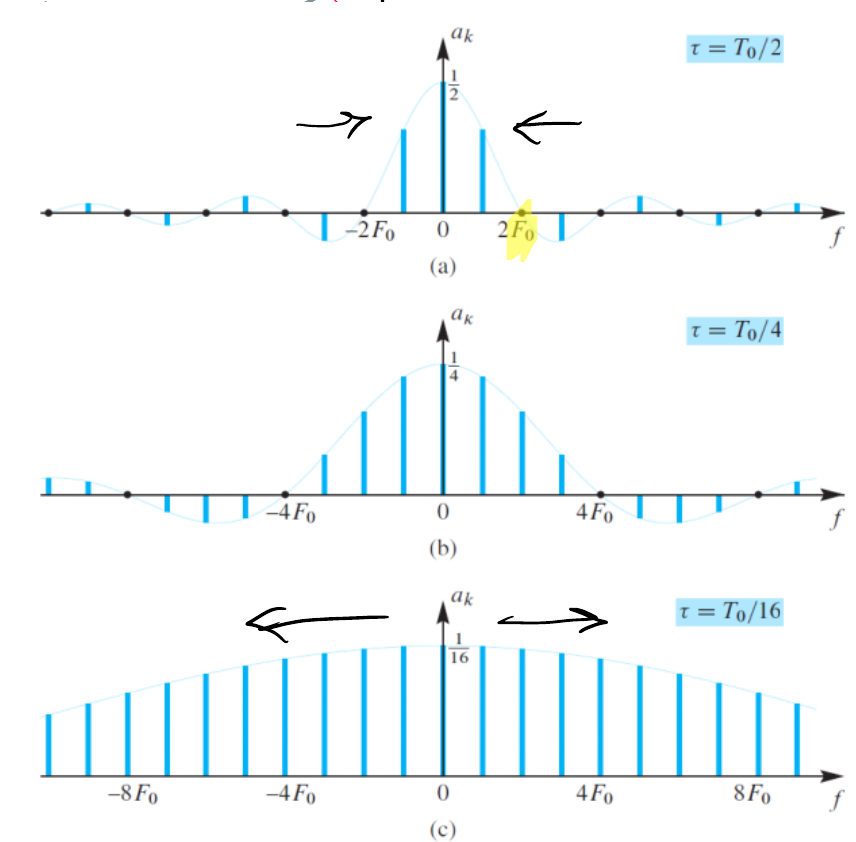
\includegraphics[scale=0.40]{immagini/lez6/manipolazionePulseWave.jpg}
\end{figure}

Introduciamo la definizione di seno cardinale (SINC) in modo da poter riscrivere la serie di Fourier in termini del seno cardinale:

\begin{equation}
    sinc(t) =
  \begin{cases}
    1 & \text{se } t = 0 \\
    \frac{\sin{(t)}}{t}   & \text{se } t \neq 0 
  \end{cases}
\end{equation}

Possiamo quindi riscrivere il segnale Pulse Wave:

\[
    x(t) = \sum_{k = - \infty}^{+ \infty} sinc(\pi F_0 k \tau) e^{-i2 \pi t k F_0}
\]

\section{Ricostruzione (sintesi o troncamento) parziale della serie di Fourier}
Sappiamo che il teorema di Fourier garantisce:
\[
    x(t) = \sum_{k = - \infty}^{+ \infty} a_k e^{-i2 \pi t k F_0}
\]

ci chiediamo ora cosa succede quando sommiamo non da meno a piu' infinito ma da $-N$ a N (non tronchiamo mai in modo asimmetrico, quindi prendiamo gli opposti).

\[
   \Tilde{x}(t) = \sum_{k = -N}^{N} a_k e^{-i2 \pi t k F_0}
\]

Come quantifichiamo un errore nel troncamento?

\subsection{Errore Massimo}
\[\begin{split}
    E_{MAX} = &MAX|x(t) - \Tilde{x}(t)| \\
    &t \in [0; T_0)
\end{split}\]

Quindi l'errore massimo e' la differenza tra il segnale originale ed il segnale ricostruito tramite la serie di Fourier con N termini.
Ovviamente l'errore variera', ma se $x(t)$ contiene una o piu' discontinuita' finite, allore l'errore massimo sara' di circa il $9\%$ dell'ampiezza della discontinuita'. Questa proprieta' si chiama fenomeno di Gibbs, ed e' presente solo se il segnale contiene una o piu' discontinuita' finite.

\subsection{Errore (quadratico) medio}

Come in statistica calcoliamo l'errore quadratico medio (varianza).

\[
    \epsilon_M^2 = \frac{1}{T_0} \int_0^{T_0} |x(t) - \Tilde{x}(t)|^2 dt
\]

Dividiamo per $T_0$ per fare la media degli errori, inoltre ricordiamo che dobbiamo fare l'integrale perche' e' il modo di sommare nei tempi continui.

L'errore medio non ci da informazioni sull'errore massimo, quindi ipoteticamente potrebbe esserci sempre un errore basso e poi in un istante un errore altissimo, il segnale medio non ci da informazioni su questa cosa.

\subsubsection{Teorema di Parseval (legge di conservazione)}
Ci serve questo teorema per poi trovare un modo per quantificare l'errore medio.
In pratica mette in relazione l'integrale del quadrato del segnale con la somma dei coeficenti della serie di Fourier, quello che facciamo e' passare dal dominio del tempo al dominio delle frequenze.

\begin{equation}
    \frac{1}{T_0} \int_0^{T_0} |x(t)|^2 dt = \sum_{k = - \infty}^{+ \infty} |a_k|^2
\end{equation}

Il primo termine e' la potenza di un segnale tempo continuo a periodico, mentre gli $a_k$ sono i coeficenti della serie di Fourier, che quindi implicitamente deve esistere.

\subsection{Errore quadratico medio con Parseval}

A questo punto posso riscrivere l'errore quadratico medio, che ricordiamo essere:

\[
    \epsilon_M^2 = \frac{1}{T_0} \int_0^{T_0} |x(t) - \Tilde{x}(t)|^2 dt
\]

utilizzando il teorema di Parseval, trasformando quindi l'integrale in sommatoria dei coeficienti, posso riscrivere il segnale:

\[\begin{split}
    x(t) &= \sum_{k = - \infty}^{+ \infty} a_k e^{-j2 \pi t F_0 k} \\
    \Tilde{x}(t) &= \sum_{k = -N}^{+ N} a_k e^{-j2 \pi t F_0 k} \\
    e(t) &= \sum_{k = - \infty}^{+ \infty} a_k e^{-j2 \pi t F_0 k} - \sum_{k = -N}^{+ N} a_k e^{-j2 \pi t F_0 k}
\end{split}\]

Facendo la differenza tra le due sommatorie, dato che i coeficienti con N saranno uguali in tutte e due le sommatorie, facendone la differenza e' come se tenessimo tutti i termini da $-\infty \rightarrow N$ e da $N \rightarrow +\infty$:

\[
    \sum_{k = - \infty}^{-N -1} a_k e^{-j2 \pi t F_0 k} - \sum_{k = N+1}^{+ \infty} a_k e^{-j2 \pi t F_0 k}
\]

Lo spettro del segnale sara':

\[
    e(t) =
  \begin{cases}
    0 & \text{se } -N \le K < N \\
    a_k   & \text{Altrimenti } 
  \end{cases}
\]

Concludendo l'errore quadratico medio nella sintesi parziale e' pari alla somma del modulo quadro dei coeficienti $a_k$ (della serie di Fourier) scartati.

Anche nel fuzzy wave i coeficenti tendono a 0, quindi l'errore medio diminiusce man mano che i coeficienti aumentano (sommo piu' segnali).

Nel segnale del seno rettificato l'errore medio e':

\[
    |\sin{(\frac{2\pi t}{T_s})}| \rightarrow \lim_{x\to\infty} |a_k| \approx \frac{1}{k^2}
\]

mentre nel segnale fuzzy wave:

\[
    a_k \approx \frac{1}{k}
\]

\section{Collocamento}
Parliamo di collocamento temporale nel senso in cui un segnale si dice ben collocato nel tempo se succede in un tempo molto piccolo, ad esempio un esplosione. Mentre un evento (segnale) si dice non collocato nel tempo se succede per la maggior parte del tempo, ad esempio la luce durante la giornata.

Quello che ci interessa e' che se il segnale ha un collocamento stretto (e' un evento in un tempo piccolo) allora serviranno tante frequenze per descriverlo, viceversa se largo.
Questa cosa l'abbiamo notata cambiano di duty cicle del segnale fuzzy wave, notando che piu' era alta piu' l'ampiezza del segnale diminuiva, e viceversa.

\section{Dualita' tempo-frequenza}
Partiamo parlando di come nei secoli l'uomo ha voluto scrivere la musica per poterla trasportare, lo facciamo rappresentando le note (che sono un suono), indicandone graficamente la frequenza e la durata:

\begin{figure}[ht!]
    \centering
    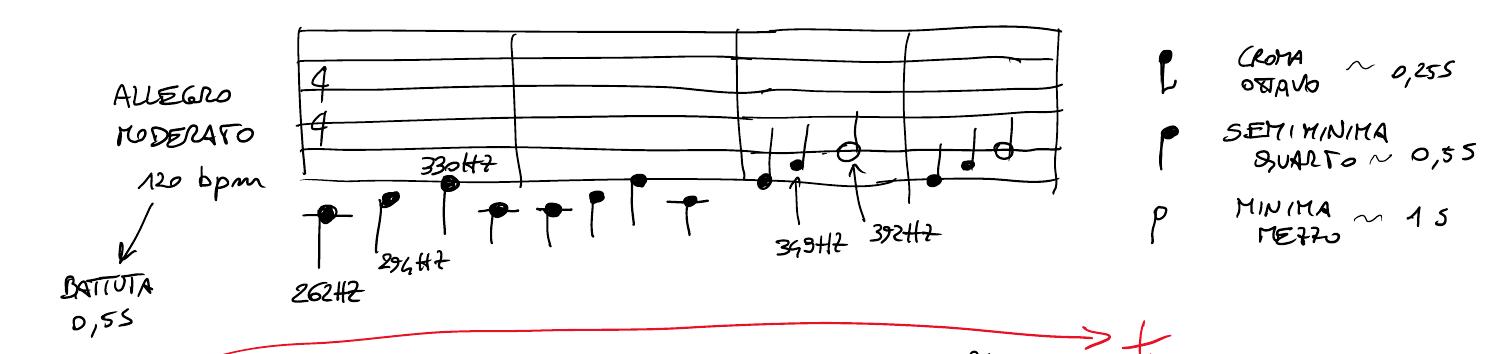
\includegraphics[scale=0.35]{immagini/lez7/campanaro.jpg}
\end{figure}

Dello spartito possiamo rappresentare il grafico del modulo (dello spettro dei segnali), e vedere come cambiano i moduli nel tempo:

\begin{figure}[ht!]
    \centering
    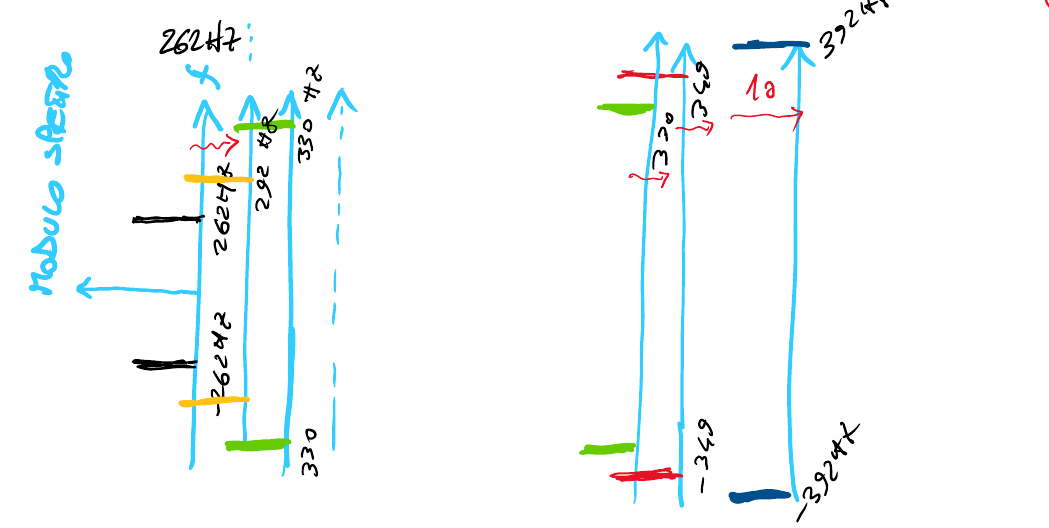
\includegraphics[scale=0.35]{immagini/lez7/graficoModuloTempo.jpg}
\end{figure}

Da quello che abbiamo visto fino ad ora possiamo rappresentare in forma trigonometrica qualisasi nota, ad esempio il DO:

\[
    A \cos{(2\pi 262 \cdot t)}
\]

Dove A e' l'ampiezza del segnale, in quando potremmo suonare un DO piu' o meno forte, mentre l'argomento del coseno e' il segnale emesso da uno strumento musicale. Pero' rappresentato in questo modo durerebbe all'infinito, cosa che intuitivamente sappiamo non essere possibile in realta', quindi prima o poi deve fermarsi.
Cio'nonostante noi possiamo considerare il segnale emesso in un preciso istante e considerarlo come se fosse infinito.

Quello che dobbiamo fare per rappresentare il segnale e' aggiungere una dimensione, il tempo e per farlo dobbiamo ricondurre il segnale al suo spettro, perche' sappiamo essere il tempo e lo spettro duali ma in due dimensioni diverse.

La rappresentazione di come evolve lo spettro di un segnale nel tempo e' detta \textbf{spettrogramma}.
Ogni trattino e' quanto dura il segnale nel tempo.

\begin{figure}[ht!]
    \centering
    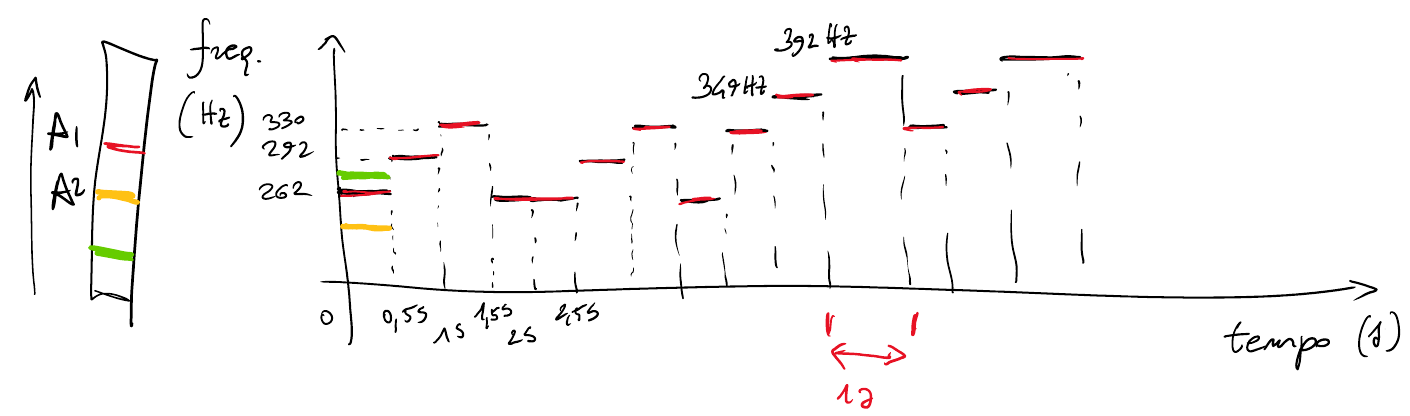
\includegraphics[scale=0.35]{immagini/lez7/spettrogramma.jpg}
\end{figure}

\section{Frequenza Istantanea}

Fino ad ora sapevamo che un segnale $\cos{2\pi f t}$ ha frequenza $f$ (ovvero le ripetizioni nel tempo). Vediamo ora dopo aver capito che dobbiamo considerare un segnale in un istante la definizione di frequenza istantanea:

\begin{equation}\begin{split}
    f_{ISTANTANEA} &= \frac{d \Theta(t)}{dt} \cdot \frac{1}{2\pi} \mbox{[Hz]} \\
    \mbox{Segnale} &= \cos{[\Theta(t)]}
\end{split}\end{equation}

Quello che dobbiamo fare in pratica e' la derivata della fase del segnale e dividerla per $2\pi$. La fase e' l'argomento nel tempo del coseno (tutto quello tra parentesi del coseno).

Dimostriamo che la definizione di frequenza istantanea coincide con quello che abbiamo fatto fino ad adesso, calcoliamo quindi la frequenza istantanea di un segnale fisso nel tempo (notiamo che $\phi = 0$ perche' il segnale non varia):

\[\begin{split}
    x(t) &= \cos{(2\pi f_0 f+ \phi)} \\
    f_{ISTANTANEA} &= \frac{d(2\pi f_0 t + \phi)}{dt} \cdot \frac{1}{2\pi} = 2\pi f_o - \frac{1}{2\pi} = f_0 
\end{split}\]

Facciamo variare adesso la frequenza istantanea nel tempo, e cerchiamo di costruire un segnale a partire dalla frequenza.

\begin{figure}[ht!]
    \centering
    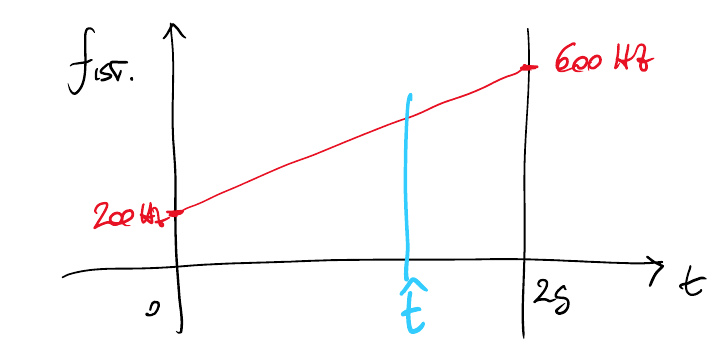
\includegraphics[scale=0.35]{immagini/lez7/fIstantaneaTempo.jpg}
\end{figure}

Dobbiamo partire dalla frequenza istantanea e costruire la fase del segnale che modula la frequenza nel tempo.
La frequenza istantanea e' l'equazione della retta (dove t e' la variabile):

\[
    f_{ISTANTANEA} = 200 + t \frac{600 - 200}{2}
\]

Ora per calcolare la fase moltiplico l'integrale tra 0 e t della frequenza istantanea per $2\pi$.

Dalla definizione precedente:

\[\begin{split}
    \Theta(t) &= \int_0^t 2\pi f_{IST} (\tau) d\tau \\
    \Theta(t) &= 2\pi \int_0^t [200 + 200 \tau] d\tau \\
    \Theta(t) &= 2\pi [200\tau + 200 \frac{\tau^2}{2}]_0^t = 200\pi [2t+t] \\
    \Tilde{x}(t) &= A \cos{[200 \pi (2t + t^2)]}
\end{split}\]

Ricordiamoci sempre che la fase non si fa mettendo direttamente la frequenza istantanea nel coseno, ma va prima integrata!

\section{Modulazione di frequenza}
Avevamo gia' visto la modulazione di ampiezza (AM), in cui il segnale trasmesso e' uguale al segnale da trasmettere moltiplicato per una portante:

\[
    x(t) = s(t) \cos{(2\pi f_0 t)}
\]

Nel caso della modulazione di frequenza (FM), ci aspettiamo che il segnale abbia un'ampiezza costante, e modulando la fase si trasmette il segnale:

\[\begin{split}
    x(t) &= a \cos{()\Theta(t)} \\
    f_{IST} &= s(t) D + F_c \\
    \Theta(t) &= 2\pi \int_0^t (s(\tau) D + F_c) \tau \rightarrow F_c >> s(t)
\end{split}\]

$F_c$ e' chiamata frequenza carrier (portante), serve per aumentare la frequenza del segnale in modo da limitare le interferenze ed e' la frequenza a cui ci sintonizziamo per ascoltare la radio. Inoltre moltiplichiamo per un'altra costante D nel caso in cui il segnale sia troppo piccolo per aumentarne l'ampiezza.


\section{Prodotto scalare di due funzioni periodiche}
Il prodotto scalare di due funzione periodiche, di periodo $T_0$:

\[
    <f(t), g(t)> \frac{1}{T_0} \int_0^{T_0} f(t) g^*(t) dt
\]

Quindi potro' dire che due funzioni sono ortogonali quando il loro prodotto scalare e' zero.

\subsection{Esempio}
Vediamo ora un esempio, calcolare il prodotto scalare tra:
\[
    <e^{i2\pi t F_o k_1}, e^{i2\pi t F_o k_2}> \rightarrow T_0 = \frac{1}{F_0}
\]

Possiamo dividere il problema in due casi, quando $k_1 = k_2$:

\[\begin{split}
    \frac{1}{T_0} &\int_0^{T_0} e^{i2\pi t F_o k} \cdot e^{-i2\pi t F_o k} dt \rightarrow = e^0 = 1 \\
    \frac{1}{T_0} &[t]_0^{T_0} = \frac{T_0}{F_0} = 1
\end{split}\]

invece quando $k_1 \neq k_2$:
\[\begin{split}
    \frac{1}{T_0} &\int_0^{T_0} e^{i2\pi t F_o k_1} \cdot e^{-i2\pi t F_o k_2} dt \\
    &\mbox{riscrivendo l'argomento dell'integrale:} \\
    &e^{i2\pi t F_0(k_1 - k_2)}\\
    &\mbox{applichiamo la formula di risoluzione dell'integrale:}\\
    \frac{1}{T_0} &[\frac{e^{i2\pi t F_0(k_1 - k_2)}}{i2\pi F_0(k_1 - k_2)}]_0^{T_0} \\
    &\mbox{risolvendo ora tra gli estremi e semplificando otteniamo:}\\
    1 &[\frac{e^{i2\pi t F_0(k_1 - k_2)}-1}{i2\pi (k_1 - k_2}] \\
\end{split}\]

Notiamo pero' che $k_1 - k_2$ sara' sempre un numero intero $\neq 0$. Quindi l'esponenziale $e^{i2\pi h} = 1$, che sottraendo con l'uno al numeratore dara' sempre 0, qualsiasi siano i valori di $k_1, k_2$.

Capito che :
\[\begin{split}
    <e^{i2\pi t F_o k_1}, e^{i2\pi t F_o k_2}> = 
    \begin{cases}
    1 & \text{se } k_1 = k_2 \\
    0   & \text{se } k_1 \neq k_2 
  \end{cases}
\end{split}\]

ci rendiamo conto che queste funzioni si comportano come somma delle basi di uno spazio vettoriale.
In uno spazio vettoriale 3D la base ortogonale standard e' composta da 3 vettori:$\Vec{i} = [100]$, $\Vec{j} = [010]$, $\Vec{k} = [001]$. Il prodotto scalare di un vettore della base con un'altro della stessa base da sempre 0, ed il prodotto scalare di un vettore della base con se stesso da sempre 1. Esattamente come succedeva per le funzioni in esempio.

Nello spazio di Fourier (le frequenze) di un segnale periodico a tempo continuo abbiamo imparato che hanno le stesse proprieta' di una base ortogonale, la differenza e' che le funzioni nello spazio di Fourier sono infinite. Come facevamo per i vettori possiamo quindi proiettare (proiezione ortogonale) ciascuna funzione sulla base e poi ricostruirla.